Salgssystemet fungerer først og fremmest via et Kasseapparat med et grafisk touch interface, herfra kan en Ekspedient sælge varer til en eventuel kunde og tage imod betaling herfra. 

Kasseapparatet sender/henter data til/fra en Central server der yderligere kommunikere med en database, dette gør at Kasseapparatet kan modtage et produktkatalog fra-, og få gemt et salg i databasen. 

Der findes derudover en Superbruger der igennem et grafisk interface har adgang til Administrationssystemet. Herfra kan Superbrugeren tilføje, slette og redigere produkter og produktkategorier i produktkataloget. Dette betyder at Administrationssystemet også har en forbindelse til Central server.

Central server sørger for alt kommunikation med databasen og at håndterer alt kommunikation til og fra alle instanser af Administrationssystem og Kasseapparat.


\begin{figure}[!h]
    \centering
    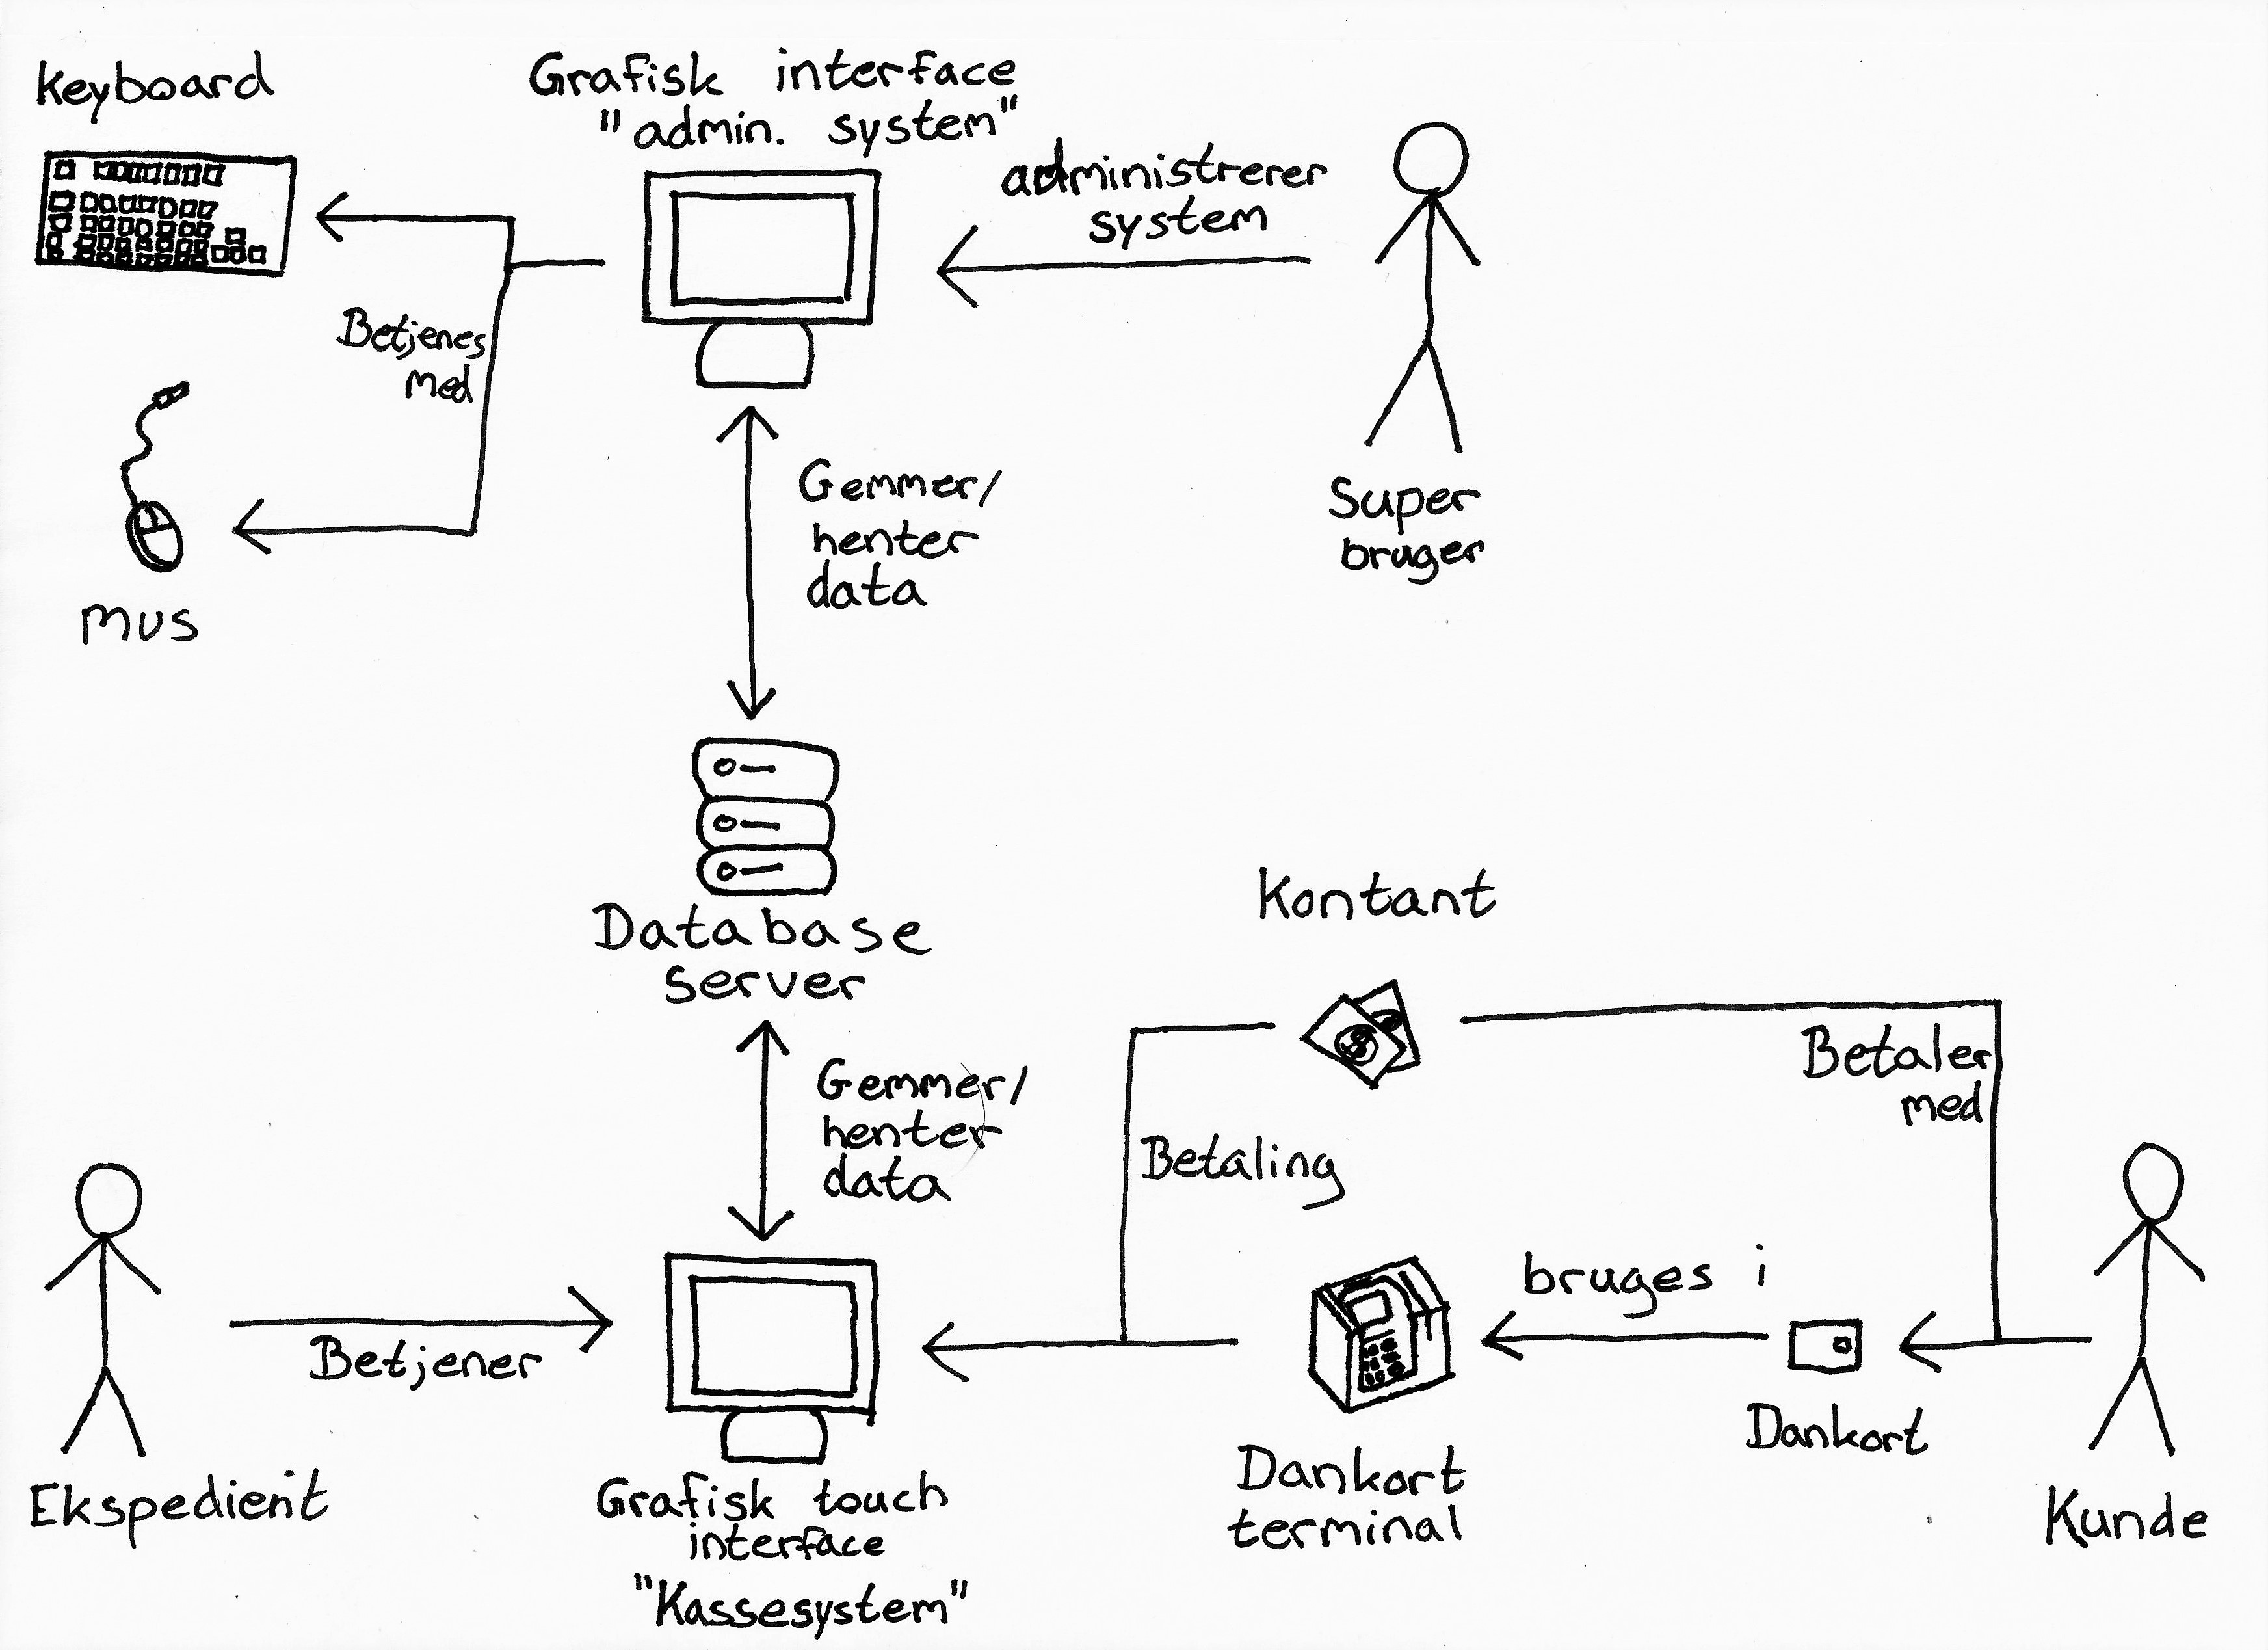
\includegraphics[width=1.0\textwidth]{Systembeskrivelse/RigtBillede2.jpg}
    \caption{Rigt billede over Salgssystemet}
    \label{fig:Rigtbill}
\end{figure}

